%\documentclass{sigplanconf}
\documentclass[preprint]{sigplanconf}

\usepackage{amsmath}
\usepackage{amssymb}
\usepackage{textcomp}
\usepackage[usenames]{color}
\usepackage{graphicx}
\usepackage{url}
\usepackage{rotating}
\usepackage{multirow}
\usepackage{booktabs}
\usepackage{listings}
\usepackage{array}
\usepackage[T1]{fontenc}
\usepackage{luximono}

\newenvironment{packed_enum}{
\begin{enumerate}
  \setlength{\topsep}{0pt}
  \setlength{\itemsep}{2pt}
  \setlength{\parskip}{0pt}
  \setlength{\parsep}{0pt}
}{\end{enumerate}}

\newenvironment{packed_itemize}{
\begin{itemize}
  \setlength{\topsep}{0pt}
  \setlength{\itemsep}{2pt}
  \setlength{\parskip}{0pt}
  \setlength{\parsep}{0pt}
}{\end{itemize}}

\newcommand{\todo}[1]{{\color{red} \bf [TODO: #1 ]}}


\lstdefinelanguage{Scala}{
  morestring=[b]",
  morestring=[b]',
  morecomment=[l]{//},
  morecomment=[s]{/*}{*/},
  morekeywords={var,val,def,private,class,object,trait,implicit,if,else,new,do,while,@volatile,try,catch,case,match,throw,return,extends,with,import}
}

\lstset{
  language=Scala,
%  basicstyle=\fontsize{7.5}{9}\selectfont\tt,
  basicstyle=\fontsize{7}{8}\selectfont\tt,
%  basicstyle=\selectfont\tt,
  keywordstyle=\bfseries,
  numbers=left,
  numberstyle=,
  commentstyle=\itshape,
  columns=fixed,
  xleftmargin=0.25in,
  firstnumber=auto,
  escapechar=\#,
  emph={A,B,C,K,V,U,Z}, emphstyle=\bfseries\itshape,
  emph={[2]Unit,Int,Set,Map,TSet,TMap,TVar,Option,Boolean,Txn,Money,Account,OverdraftException,Ref,Source,Sink,Bound,ReadResource}, emphstyle={[2]\itshape}
}

\newcommand{\code}[1]{{\fontsize{8}{9.5}\selectfont \tt #1}}
\newcommand{\codesec}[1]{{\fontsize{10}{12}\selectfont \tt \bfseries #1}}
\newcommand{\codeft}[1]{{\fontsize{6.5}{8}\selectfont \tt #1}}
\newcommand{\type}[1]{{\code{\itshape #1}}}
\newcommand{\typesec}[1]{{\codesec{\itshape #1}}}
\newcommand{\typeparam}[1]{{\code{\bfseries #1}}}
\newcommand{\typeparamsec}[1]{{\codesec{\bfseries #1}}}
\newcommand{\xtype}[2]{{\type{#1}\typeparam{[#2]}}}
\newcommand{\xtypesec}[2]{{\typesec{#1}\typeparamsec{[#2]}}}
\newcommand{\ytype}[2]{{\type{#1}\code{[}\type{#2}\code{]}}}
\newcommand{\xxtype}[3]{{\type{#1}\typeparam{[#2,#3]}}}
%\newcommand{\keyword}[1]{{\code{\bfseries #1}}}
\newcommand{\keyword}[1]{{\code{#1}}}

\hyphenation{CC-STM}
\hyphenation{Deuce-STM}
\hyphenation{Mul-ti-verse}

\begin{document}

\conferenceinfo{Scala Workshop,}{April 15, 2010, Lausanne, Switzerland.}
\CopyrightYear{2010}
\copyrightdata{}

\newcommand{\xtitle}[0]{CCSTM: A Library-Based STM for Scala}
\newcommand{\xterms}[0]{{Algorithms, Languages}}
\newcommand{\xkeywords}[0]{{Transactional memory, Scala}}
%\titlebanner{[WORK IN PROGRESS: Do Not Circulate!]}        % These are ignored unless
\preprintfooter{\xtitle}  % 'preprint' option specified.

\title{\xtitle}

\authorinfo{Nathan G. Bronson \and Hassan Chafi \and Kunle Olukotun}
           {Computer Systems Laboratory\\
            Stanford University}
           {\textit{\{nbronson, hchafi, kunle\}@stanford.edu}}

\pdfinfo{
  /Title    (\xtitle)
  /Author   (Nathan G. Bronson and Hassan Chafi and Kunle Olukotun)
  /Subject  (\xterms)
  /Keywords (\xkeywords)
}

\maketitle

\begin{abstract}

We introduce CCSTM, a library-only
software transactional memory (STM) for Scala, and
give an overview of its design and implementation.
Our design philosophy is that CCSTM should be a useful tool for the
parallel programmer, rather than a parallelization mechanism for arbitrary
sequential code.  This frees us from the semantic tar pits that surround
privatization, strong isolation, and irrevocable system calls.
It also allows us to express the STM using Scala classes and methods, a design
choice that has far-reaching consequences.

Transactional accesses in CCSTM are performed via explicit method calls
on instances that implement a trait \type{Ref}.  These transactional
references may be long-lived, or may be transient accessors to bulk
transactional data such as an array.  Scala's operator overloading keeps
the syntactic overhead low for basic reads and writes.  The \type{Ref}
trait serves as a first-class representation of a transactionally-managed
memory location, providing a natural way to express additional STM
functionality such as modular blocking, non-transactional compare-and-swap,
manually-validated reads, and deferrable transformation using pure
functions.

In an additional departure from typical STM designs, CCSTM uses a
hybrid of static and dynamic transaction scoping.  \type{Ref}'s methods
are bound to current transaction via a \keyword{implicit} parameter.
When an atomic block is entered, however, nesting is resolved dynamically.
This hybrid approach avoids the overheads of a dynamic lookup for most
STM operations without requiring the transaction to be statically threaded
throughout the user's code.

\end{abstract}

\category{D.1.3}{Programming Techniques}{Concurrent Programming -- Parallel programming}
\category{D.4.1}{Operating Systems}{Process Management -- Concurrency; Synchronization; Threads}

\terms
\xterms

\keywords
\xkeywords

\section{Introduction}
\label{sec:intro}
The proliferation of multi-core processors means that more programmers are
being thrust into the difficult world of shared memory multi-threading.
Software transactional memory (STM) provides a compelling alternative to
locks for managing access to shared mutable state; STM's declarative
atomic blocks are free from deadlock, are composable, and do not
require elaborate fine-grained decomposition to yield scalability.

%The benefits of memory transactions stem from an optimistic execution
%strategy that includes rollback and retry.  The ability to recover from
%error allows the runtime to
%attempt concurrent execution without a guarantee that it is possible.
%STMs bridge the gap between their simple programming model and their
%speculative execution by isolating uncommitted transactions from the
%rest of the system.  Most of the difficulty in integrating an STM into
%a language comes from tradeoffs between the overhead, fidelity, and
%complexity of this isolation.

In this paper we describe the design of CCSTM, a library-based STM
for Scala.  CCSTM deliberately sidesteps many of the 
semantic difficulties common in software implementations of transactional
memory, by limiting its focus: we view CCSTM as a domain-specific language
for use by parallel programmers that wish to build algorithms and data
structures using optimistic concurrency control.  CCSTM is not a drop-in replacement for
locks, an all-encompassing concurrent programming model, or a mechanism
for automatic parallelization of arbitrary code.

The most fundamental design choice for CCSTM was the decision to
implement it entirely as a Scala library.  Unlike STMs that transparently
instrument
all loads from and stores to shared mutable state, transactional accesses in CCSTM are explicit
method calls to a Scala \keyword{trait}\footnote{Custom accessor methods
may used to eliminate the syntactic overhead for some situations.}.
We refer to the resulting STM as `reference-based', because all memory
locations managed by the STM are boxed inside transactional references.
Both transactional and non-transactional access to the managed references
goes through methods implemented by instances of this \xtype{Ref}{A}.

While a reference-based STM imposes a syntactic burden for simple loads and
stores, it also provides advantages.  Encapsulating transactionally-managed
data eliminates the weak isolation issues that plague transparent STMs.
The \type{Ref} provides
a first-class object that names a memory location, which enables the
expression of higher-level constructs such as a simple but effective form of
semantic conflict detection.
The reference also provides a convenient
namespace for additional STM functionality.
%As a
%practical benefit, the extra level of indirection provided by \type{Ref}
%allows multiple implementations, allowing tradeoffs between the cost of
%validation and the likelihood of rollback.

CCSTM's second departure from the typical STM interface is that it binds the
transaction scope statically, rather than dynamically.  Transactional access
methods in \type{Ref} take an implicit parameter of type \type{Txn}, and
perform their accesses in the context of that transaction.
%This decision
%was made for pragmatic reasons, because performing a dynamically-scoped
%lookup on each transactional access would be prohibitively expensive.
A useful parallel can be made between Haskell's STM~\cite{harris05composable} and CCSTM.
Haskell's \type{TVar} corresponds to instances of type \type{Ref}.
\type{Txn} is not a monad, but it proliferates through STM-enabled
methods in exactly the same way as the \type{STM} monad.

In this paper:
\begin{packed_enum}

\item We describe CCSTM, a reference-based STM for Scala.  CCSTM focuses on
helping parallel programmers build optimistically concurrent algorithms
and data structures, while restricting itself to implementation techniques
that do not interfere with components of the system that do not use it
(Section~\ref{sec:ref}).

\item We introduce \code{unrecordedRead}, a new STM primitive that relaxes
read atomicity while allowing manual validation, and \code{map}, a simple
and safe way of expressing semantic conflict detection.  A transaction
that reads a refrence \code{x} via \code{x.map(f)} does not need to roll
back if \code{x} is changed concurrently but \code{f(x.get)} remains
the same (Sections~\ref{sec:unrecordedread} and~\ref{sec:map}).

\item We summarize the discussions that led from the original design goal to
the current syntax.  We point out the parts that work well and the parts that
are burdensome, and hypothesize about ways to address the latter
(Section~\ref{sec:syntax}).

\item We compare the performance of CCSTM to DeuceSTM, an STM for
the JVM that use bytecode rewriting~\cite{deucestm}.
We find that CCSTM's implementation as an
unprivileged library does not impose a significant performance penalty
(Section~\ref{sec:perf}).

\end{packed_enum}



\begin{figure}
\begin{lstlisting}{name=Code}
class Account(initialBalance: Money) {
  private var _balance = initialBalance

  def balance: Money = _balance

  def deposit(amount: Money): Unit = {
    assert(amount >= 0)
    _balance += amount
  }

  def withdraw(amount: Money): Unit = {
    assert(amount >= 0)
    if (_balance < amount)
      throw new OverdraftException
    _balance -= amount
  }
}

object Account {
  def transfer(src: Account, dst: Account,
        amount: Money): Unit = {
    src.withdraw(amount)
    dst.deposit(amount)
  }
}
\end{lstlisting}

\caption{Code that performs an account transfer without
any locking or other concurrency control.}

\label{fig:example:nosync}
\end{figure}


\section{Motivation}
\label{sec:library}

An experimental feature such as software transactional memory should strive to
impose only neglible costs on code that does not use it.  Runtime performance
costs are the most obvious, but software engineering costs in the compiler and
language implementation are also important.

\subsection*{Strong Isolation}

At its most basic, a software transactional memory is a way of isolating
a group of memory accesses and verifying that those accesses are
equivalent to some serial execution.  The STM manages reads and writes
by redirecting them to \textit{barriers}, code fragments that actually
implement the atomicity and isolation.  These properties can only be
guaranteed, however, if no non-transactional code bypasses the barriers
and accesses a memory location directly.

There are three potential responses to the weak isolation between direct memory
accesses and concurrent transactions:
\begin{packed_itemize}

\item The system can provide strong isolation and atomicity by redirecting
all memory accesses to barriers, even non-transactional accesses.  While
there has been some research in using dynamic recompilation to reduce the
performance penalty of strong isolation, deep integration with the VM's
JIT is required to achieve acceptable performance~\cite{inteldbo,mydbo}.

\item The system can declare that a conflicting concurrent access
from both inside and outside a transaction is an error.  This doesn't
sound too onerous, but the optimistic nature of transactions means
that failed speculations must also be considered: inconsistent
transactions may execute conflicting accesses from an impossible
branch, or they may execute conflicting accesses after they have become
doomed~\cite{grossman?get-cite-from-my-dbo}.  Restrictions on commit
order can prevent some of the most surprising behaviors, but there is
a substantial performance penalty to restoring even the race semantics
of locks~\cite{sgla}.

\item The system can use the type system to disallow direct access to
any memory location that might be touched transactionally.  In one
variation on this theme the type system disallows non-transactional
accesses entirely, in another it uses the type system to identify memory
locations that must be accessed via non-transactional
barriers~\cite{smallstepsemantics,cmt}.  Haskell~\cite{cmt} and 
Clojure~\cite{?} both adopt this approach.

\end{packed_itemize}

Scala 

These properties are only guaranteed, however, if
the STM manages all accesses to a memory location used in a transaction.
there are no direct non-transactional accesses to these memory locations.
This can cause 

Many STMs transparently redirect normal loads
and stores to barriers when they are executed within the dynamic scope of
a transaction.  This implicit interface has the advantage of leveraging
the language's syntax for loads and stores, which is almost always highly
optimized and concise.


in all successful
languages.

highly optimized syntax
available in 
that are executed within the dynamic scope of a transaction.

read bTo manage memory accesses, the STM intercepts
them with \textit{read barriers} and \textit{write barriers}.  The STM can only
maintain the illusion of isolation and atomicity for accesses that use
barriers, however, so problems 


The
most common STM operations in an atomic block are reads and writes, so their
invocation syntax has a large impact on the clarity of the code.  Many STMs
transparently redirect 


One way of
categorizing STMs is by how barriers are invoked

When integrating an STM into a language, one of the most fundamental
questions is, "How are the barriers invoked?" Because the most common
operations in an STM are reads and writes, their syntax has a large impact
on the resulting code.  Scala, like virtually all programming languages,
has a very concise and refined syntax for accessing memory.  The most
streamlined syntax for invoking transactional read and write barriers
would be to piggyback on the basic read and write syntax, transparently
redirecting all memory accesses through the STM.

While transparent barriers provide a convenient syntax, they introduce the
potential for weak isolation.  If transactional access is provided to all
fields and array elements, then the STM 

When designing CCSTM,
however, we chose not to provide transparent transactional barriers.



Integrating an experimental feature such as STM into an existing full-featured
language is difficult, especially for a language like Scala that provides
excellent performance.  The new feature must provide benefits, without 
imposing a burden on code that doesn't use it.

provide full benefits for code
that uses it without imposing any burden on existing code and code that does

One of the
fundamental questions when integrating an STM into a language is how these
barriers are invoked.  There are four reasonable strategies for Scala.  In the
first three, field and array element accesses are transparently redirected to
barriers:
\begin{packed_enum}

\item Execute on a VM whose JIT compiler has been extended to emit
transactional read and write barriers when compiling field and array element
accesses.

\item Perform bytecode rewriting during class loading, replacing field and
array element instructions with method calls or inline code sequences that
implement the barriers.

\item Add barrier invocations during compilation from Scala to bytecode.

\item Require that the programmer call barrier methods, rather than perform
field or array element reads and writes.

\end{packed_enum}

STMs often attempt to mimic the syntax used for lock-based critical
regions.  The beginning and end of the atomic block are declared, and all
memory accesses that occur within the dynamic scope of the atomic block
are transparently redirected to read or write barriers.  This has the
advantage that transactional accesses inherit the programming language's
syntax for reads and writes, which is both concise and familiar.
This familiarity is both a blessing and a curse, however.  It creates an
expectation that the STM can safely execute arbitrary existing sequential
code, which creates both semantic and performance challenges, and it
makes it more difficult for the programmer to convey semantic information
to the STM, which reduces opportunities for compile-time checking and
run-time scalability and performance improvements.

A Scala STM implemented inside the VM's JIT is likely to have the best
performance.  Past research has identified profitable transformations
that can be made by the optimizer if it has knowledge of barrier
usage~\cite{?}.  This approach is not a pragmatic one, however, because
the engineering effort required to produce a production quality VM with
this capacity is feasible only for a few organizations.

Bytecode rewriting is a promising technique.  Several bytecode rewriting STMs
have been described for the JVM, including Multiverse~\cite{multiversewebsite},
DeuceSTM~\cite{??}, and AJ~\cite{popl09bronson}.  For Scala, this approach
has the advantage of allowing transactional execution of Java code,
including the Java standard libraries.

Bytecode rewriting has several drawbacks, however.  Because transactional
execution is dynamically scoped, it is not known at class loading time
whether or not transactional versions of an object or a method will
be required.  This means that all methods must be duplicated, adding
class loading overhead and increasing the size (and therefore decreasing
the spatial locality) of the VM's class data structures.  The bytecode
rewriter must be given special privileges, which complicates deployment
and limits the environments in which it may be used.

Instrumenting memory accesses in the Scala to bytecode compiler eliminates
execution overhead at class loading time, and it avoids the need for the STM to
be given elevated privileges, but it limits the 

by the bytecode 
a production quality 

profitable optimizations available
if the 

The dynamic scope of transactional execution in an STM with transparent barrier
invocations is also a problem, because it means that it is impossible to
determine in general whether a particular method may be invoked

transparent STMs

There are three possible strategies for implementing a Scala STM with
transparent barriers:
While this strategy is likely to yield
the best performance, such VMs are neither widely available nor production
quality.

Several STMs have been
described that perform this transition for the JVM, and therefore should be
easily adaptable to Scala.

, since it creates an expectation that the STM can
safely execute all existing sequential code.

with scoping to
guarantee pairing, 

Introducing
an STM should provide the full benefits of transactional memory for
code that uses it, without imposing a burden on existing code or syntax.
The need to isolate code executed in a transaction from the rest of the system
makes such a ``pay as you go'' STM difficult:
\begin{packed_itemize}

\item \textbf{Strong isolation:}\footnote{Strong isolation is also 
referred to as strong atomicity.} Should non-transactional memory accesses be isolated from
acceses made inside a transaction?  If so, existing code will run slower, even
if it doesn't use transactions.  If not, programmers will be exposed to a
variety of semantic pitfalls.

\item \textbf{Instrumentation overhead:} STMs 

\item \textbf{Irrevocable actions:} What happens when a transaction performs
I/O, makes a native call, or does some other action that cannot be undone?
While better alternatives may be enumerated for specific cases, a
general-purpose STM 

\item 

\end{packed_itemize}

in the decision to add STM to an existing language.


To bridge the gap between the programming model and the execution
strategy, speculative 

provides the illusion of
atomicity and isolation, while allowing 


stem from an optimistic execution model that allows speculation, rollback,
and retry.  

The STM takes responsibility for ensuring that speculative
executions are isolated from actions taken by concurrent threads.

, while isolating incorrect speculations from concurrent threads.
Isolating 

Software transactions
solve the deadlock and composability problems inherent in pessimistic
locking, while at the same time presenting a simpler interface to the
programming.


%\section{\xtypesec{Ref}{A} and \xtypesec{Ref.Bound}{A}}
\section{The Basic Interface}
\label{sec:ref}
As a recurring example of the ways in which CCSTM allows optimistic concurrency
to be expressed, consider a class that encapsulates the balance of a
checking account\footnote{This example is from the bank benchmark included
in DeuceSTM~\cite{deucestm}.}.  Absent any concurrency control, we might
write the code in Figure~\ref{fig:example:nosync}.  (Here \type{Money}
is an immutable numeric type suitable for representing quantities of
a currency.)  Adding pessimistic concurrency control to this code by
locking accesses to \type{Account} instances is not straightforward,
because both the source and destination account must be locked during
a \code{transfer}.  Unless a global lock order is followed this can
easily lead to deadlock.

\begin{figure}
\begin{lstlisting}{name=Code}
class Account(initialBalance: Money) {
  private var _balance = initialBalance

  def balance: Money = _balance

  def deposit(amount: Money): Unit = {
    assert(amount >= 0)
    _balance += amount
  }

  def withdraw(amount: Money): Unit = {
    assert(amount >= 0)
    if (_balance < amount)
      throw new OverdraftException
    _balance -= amount
  }
}

object Account {
  def transfer(src: Account, dst: Account,
        amount: Money): Unit = {
    src.withdraw(amount)
    dst.deposit(amount)
  }
}
\end{lstlisting}

\caption{Code that performs an account transfer without
any locking or other concurrency control.}

\label{fig:example:nosync}
\end{figure}

\begin{figure}
\begin{lstlisting}{name=Code}
class Account(initialBalance: Money) {
  private val _balance = Ref(initialBalance)

  def balance: Source[Money] = _balance

  def deposit(amount: Money
        )(implicit txn: Txn): Unit = {
    assert(amount >= 0)
    _balance := !_balance + amount
  }

  def withdraw(amount: Money
        )(implicit txn: Txn): Unit = {
    assert(amount >= 0)
    if (!_balance < amount)
      throw new OverdraftException
    _balance := !_balance - amount
  }
}

object Account {
  def transfer(src: Account, dst: Account,
        amount: Money): Unit = {
    new Atomic { def body {
      src.withdraw(amount)
      dst.deposit(amount)
    }}.run()
  }
}
\end{lstlisting}

\caption{One way to implement the atomic balance transfer function
using CCSTM.  This code uses \code{unary\_!} and \code{:=} operators
(ML-inspired) for performing transactional reads and writes, and
expresses the atomic block by extending \code{Atomic}.}

\label{fig:example:ccstm}
\end{figure}

CCSTM allows the atomic balance transfer to be expressed easily,
guaranteeing that both balance adjustments are performed atomically and
without deadlock.  Figure~\ref{fig:example:ccstm} gives the transactional
code.

\subsection{References -- \xtype{\bfseries Ref}{A} and \xtype{\bfseries Ref.Bound}{A}}

The most fundamental data type in CCSTM is \xtype{Ref}{A}, which mediates
access to an STM-managed mutable value.  Read-only methods are separated into a
covariant \type{Source} trait and write-only methods are separated into a
contravariant \type{Sink} trait.  The current transactional context is passed
during
each method call via an implicit parameter.  Reads and writes on a
reference may be performed with the \code{get} and \code{set} methods,
respectively, or with the ML-inspired \code{unary\_!} and \code{:=}
operators.  Section~\ref{sec:syntax} discusses
the choice of method names in more detail.

\begin{figure*}
  \centering
  \includegraphics[clip=true,width=5.5in]{build/refs_class_uml}

\caption{Traits that provide access to an STM-managed memory
location.  Transactional access can occur through either \type{Ref}
or a \type{Ref.Bound} returned from \type{Ref}\code{.bind},
non-transactional access occurs through a \type{Ref.Bound} returned
from \type{Ref}\code{.nonTxn}.  \xtype{Source}{+A} and \xtype{Sink}{-A}
decompose the covariant and contravariant operations of \xtype{Ref}{A}.}

\label{fig:refclasses}
\end{figure*}


\begin{figure}
\textbf{Source.Bound Methods:}
\begin{packed_itemize}
\item \code{unary\_!: T} -- This is equivalent to a \code{get}.
\item \code{get : T} -- Performs a transactional read of the value 
managed by the bound Ref. If the bound view was created by nonTxn, the read will
be strongly atomic and isolated with respect to all transactions.
\item \code{map[Z](f: T => Z): Z} -- Returns \code{f(get)}, possibly 
reevaluating f to avoid rollbacks (\code{f} must be idempotent).
\item \code{await(p: T => Boolean)} -- Blocks until \code{pred} is true, in a 
manner consistent with current context (transactional vs. non-transactional).
\item \code{unrecordedRead: UnrecordedRead[T]} -- Returns an \code{UnrecordedRead} instance that 
wraps the value that would be returned by \code{get}. The read will not be added to the transaction's read set (transactional context).
\item \code{releasableRead: ReleasableRead[T]} -- Returns a \code{ReleasableRead} instance that 
wraps the value that would be returned by \code{get}. The read will be added to the transaction's read set (transactional context) but it may be removed by a call to 
\code{ReleasableRead.release()}.
\end{packed_itemize}

\textbf{Sink.Bound Methods:}
\begin{packed_itemize}
\item \code{:=(v: T)} -- This is equivalent to a \code{set}.
\item \code{set(v: T)} -- Updates the value 
\item \code{tryWrite(v: T): Boolean} -- 
\end{packed_itemize}

\textbf{Ref.Bound Methods:}

\begin{packed_itemize}
\item{This is my item}
\end{packed_itemize}

\caption{Description of methods provided by Sink.Bound, Source.Bound and Ref.Bound }
\end{figure}

Non-transactional access to the contents of a reference are provided by a view
returned by \code{nonTxn}.  This view implements methods that parallel those of
the reference, but that don't require a \type{Txn}.  We say that the view
is \textit{bound} to the non-transactional context, so the view trait is
named \type{Ref.Bound}.  Views may also be bound to a transactional context
via \type{Ref}\code{.bind}.  These bound references do not require a \type{Txn}
parameter, but may only be used until the end of the transaction.
Figure~\ref{fig:refclasses} shows the
\keyword{extends} relationship between the traits that implement unbound
and bound references, and some of their methods.  The separation between
\type{Ref}, \type{Source}, and \type{Sink}, and the operator syntax for
accesses are modeled after Spiewak's Scala STM~\cite{github:spiewak}.
The \type{Ref} $ \leftrightarrow $ \type{Ref.Bound} duality is unique
to CCSTM, as far as is known by the authors.

Bound views for non-transactional access create a syntactic difference
between transactional and non-transactional reads and writes.
This allows the expert programmer to selectively relax isolation by
performing a non-transactional access inside an atomic block, without
requiring an escape action~\cite{escapeaction}.  The non-isolated access
is visually differentiated by including the token \code{nonTxn}.  In
Section~\ref{sec:unrecordedread} we will introduce \code{unrecordedRead},
a way of relaxing isolation for reads while retaining the ability to
manually validate it.

\subsection{Declaring and executing an atomic block}

CCSTM currently provides two syntaxes for declaring atomic blocks.  The first,
shown in Figure~\ref{fig:example:ccstm}, involves extending the
abstract class \type{Atomic} and implementing the method \code{body:
}\type{Unit}.  The base class introduces an implicit \type{Txn} into the
static scope of the body, resulting in a relatively concise syntax for
inline transactions.  This form produces an extra set of curly braces
and several extra tokens, but it uses only one line to open the scope
and one to close it.  \xtype{AtomicFunc}{Z} provides a similar syntax
for atomic blocks that return a value.

The second syntax is to pass a function \type{Txn}\code{~=>~}\typeparam{Z}
to the \code{atomic} method on the \type{STM} object.  This syntax is more
concise when invoking a method.  The \type{Account}\code{.transfer} method
might be decomposed into:
\lstset{numbers=none}
\begin{lstlisting}
def transfer(src: Account, dst: Account,
      amount: Money): Unit = {
  STM.atomic(transferInTxn(src, dst, amount)(_))
}
def transferInTxn(src: Account, dst: Account,
      amount: Money)(implicit txn: Txn): Unit = {
  src.withdraw(amount)
  dst.deposit(amount)
}
\end{lstlisting}
\lstset{numbers=left}

One of the new features of Scala 2.8 is support for an \keyword{implicit}
modifier on parameters to anonymous methods (ScalaTrac ticket \#1492).
This will make \type{STM}\code{.atomic} more concise for inline
transactions, as in (with the addition of an \keyword{import}):
\lstset{numbers=none}
\begin{lstlisting}
  atomic { implicit txn: Txn =>
    src.withdraw(amount)
    dst.deposit(amount)
  }
\end{lstlisting}
\lstset{numbers=left}
This will also allow a syntax that leverages \keyword{for} comprehensions.
This syntax has a special elegance; it implies that the block may be
executed multiple times, which is exactly the essence of optimistic
concurrency!
\lstset{numbers=none}
\begin{lstlisting}
  for (implicit txn <- atomic) {
    src.withdraw(amount)
    dst.deposit(amount)
  }
\end{lstlisting}
\lstset{numbers=left}
Both of these syntaxes can be supported by an \type{atomic} object:
\lstset{numbers=none}
\begin{lstlisting}
object atomic {
  def apply[Z](body: Txn => Z): Z
  def foreach[Z](body: Txn => Z): Z
}
\end{lstlisting}
\lstset{numbers=left}

The decision to statically scope CCSTM's transactions was made for
performance reasons.  To dynamically scope the transactions, the
current transaction must be identified by each read and write barrier.
This is an extremely frequent operation.  Bytecode rewriting STMs have
two options for efficiently performing this lookup: they can add a field
to the system-wide \type{Thread} class, or they can weave a \type{Txn}
parameter into the transactional version of every method.  A library-only
STM running on the JVM must restrict itself to \type{ThreadLocal},
which navigates from the \type{Thread} to a thread-local hash table,
and from there to the dynamically scoped value.

\subsection{Conditional retry}

CCSTM supports the \code{retry} and \code{orElse} primitives introduced by
Harris et al. in Haskell's STM~\cite{harris05ctm}, although the current
lack of nesting support makes them less expressive than the original.
The \code{retry} primitive causes the surrounding transaction to be rolled
back, but retry is postponed until at least one of the values read by
the transaction has changed.  \code{orElse} combines two transactions,
attempting the second if the first calls \code{retry}, then blocking
both transactions if the second calls \code{retry}.  Intuitively, a call
to \code{retry} is a dead end; the STM will restart the transaction
only after it might take a different path.  Similarly, \code{orElse}
composes two alternatives that are each satisfactory, and requests that
whichever one can avoid the dead end should be executed.

\type{Atomic} provides a \code{retry} method.  As a contrived example,
the bank could use \code{retry} if they wished to delay a withdrawal
rather than trigger an \code{OverdraftException}:
\lstset{numbers=none}
\begin{lstlisting}
object atomic {
  def withdrawWhenPossible(amount: Money
        )(implicit txn: Txn): Unit = {
    assert(amount >= 0)
    if (!_balance < amount)
      retry
    _balance := !_balance - amount
  }
\end{lstlisting}
\lstset{numbers=left}

A chain of \type{Atomic} or \type{AtomicFunc} instances may be chained
with \code{orElse}, a single \code{run()} terminates the alternatives.
If a collection of \type{Txn}\code{~=>~}\typeparam{Z} is available then
they can be passed to:
\lstset{numbers=none}
\begin{lstlisting}
object STM {
  def retryOrElse[Z](blocks: (Txn => Z)*): Z
}
\end{lstlisting}
\lstset{numbers=left}

%Ref eq vs ==

\subsection{Additional reference operations}

\subsection{Relaxed isolation}
\label{sec:unrecordedread}

Some algorithms can benefit from transactional reads that are not
atomic, but that observe speculative stores made by the current
transaction.  The inconsistent value may be used to make a heuristic decision,
such as a hash table resize, or algorithm-specific knowledge
may be used to guarantee atomic behavior of the transaction despite
a subsequent invalidation, as in early release when searching a binary tree.

Previous TM systems have provided several mechanisms for relaxing atomicity and
isolation.
Open nested transactions~\cite{opennested} allow the actions of a
nested transaction to be committed in a non-nested fashion.  Escape actions
suspend the current transaction temporarily~\cite{escapeaction}.  Early
release
allows reads to be removed from the read set prior to
commit~\cite{HerlihyLMS03}.  CCSTM's static transaction scoping makes escape
actions trivial.  Accesses via \code{nonTxn} are escaped when executed by the
code that implements an atomic block\footnote{One of the motivations for the
creation of CCSTM was to study transactional collection class implementations
that interleave escaped actions internally.}
CCSTM also provides principled support for
early release, via \type{Source.Bound.releasableRead}.  This method returns
a \type{ReleasableRead} instance that provides both the read value
and a method that removes the access from the transaction's read set.
This interface eliminates the danger that an algorithm will remove a
read that it did not perform, but it still requires careful reasoning to
provide correctness.

As an alternative to a releasable read, CCSTM provides a new
abstraction, \code{unrecordedRead}.  This method performs a
transactional read, but instead of adding an entry to the read set it
bundles the read's meta-data into an \type{UnrecordedRead} instance.
The caller may then use this instance to manually validate that the
returned value is still valid.

Like many STMs, CCSTM performs transactional reads by associating a
version number with each managed memory location, recording the version
prior to a transactional read, and checking during validation that the
version number remains unchanged.  An \type{UnrecordedRead} contains the
read value and the prior version, but rather than automatically validating
the read during commit, validation is exposed to the programmer via the
method \code{stillValid}.  An unrecorded read is considered to still be
valid if the only changes that have been made to the referenced memory
location were performed by the read's transaction.  This definition also
provides a meaning for unrecorded reads of the \code{nonTxn} bound view:
\code{stillValid} will return true only if no change has been made to the
managed value.  This leverages the STM's meta-data to solve
the ABA problem\footnote{The ABA problem is when an observer falsely
concludes that a value has not changed, because the watched value went
from A to B, then back to A.}.

\subsection{Semantic conflict detection for reads}
\label{sec:map}

Unrecorded reads can be paired with life cycle callbacks to implement a
simple yet powerful form of semantic
conflict detection.  CCSTM's \type{Txn} allows the user to register a callback
that will be invoked whenever the transaction's read set is validated.  If
an unrecorded read is coupled with a callback that re-reads the value and
performs a semantic validation, rollback may be avoided.
We use this technique to
implement a new abstraction:
\lstset{numbers=none}
\begin{lstlisting}
trait Source[+A] {
  def map[B](f: A => B)(implicit txn: Txn): B
}
\end{lstlisting}
\lstset{numbers=left}
\code{x.map(f)} returns the same value as \code{f(x.get)}, but no rollback
is triggered if the post-application value does not change.  Without this
semantic conflict detection, the STM must initiate rollback any time \code{x}
is changed concurrently, even if that change is masked by the definition of
\code{f}.

Consider a branch that should be taken only if the transactional value of
\code{x} is greater than 100, and assume that a concurrent transaction commits
a change of \code{x} from 200 to 201:
\lstset{numbers=none}
\begin{lstlisting}
  if (x.get > 100) { ... }
\end{lstlisting}
\lstset{numbers=left}
When the comparison is performed directly by the caller, the STM must
trigger an optimistic rollback for any concurrent write to \code{x}, even
though
the outcome of the conditional check is not affected.  If the comparison is
moved inside \code{map} then no rollback is required:
\lstset{numbers=none}
\begin{lstlisting}
  if (x.map(_ > 100)) { ... }
\end{lstlisting}
\lstset{numbers=left}
By allowing the programmer to express more of his or her intention to CCSTM,
\code{map} can reduce rollbacks, leading to better performance and scalability.



\section{Advanced Functionality}
\label{sec:advanced}

\subsection{Relaxed isolation}
\label{sec:unrecordedread}

Some algorithms can benefit from transactional reads that are not atomic,
but that observe speculative stores made by the current transaction.
The inconsistent value may be used to make a heuristic decision, such as a
hash table resize, algorithm-specific knowledge may be used to guarantee
atomic behavior of the transaction despite a subsequent invalidation,
as in early release when searching a binary tree, or life cycle callbacks
may be used to provide customized validation.

Previous TM systems have provided several mechanisms for relaxing
atomicity and isolation.  Early release allows reads to be removed
from the read set prior to commit~\cite{HerlihyLMS03}.  Escape actions
suspend the current transaction temporarily~\cite{harris04exceptions}.
Open nested transactions allow the actions of a nested transaction
to be committed in a non-nested fashion.  CCSTM's static transaction
scoping makes escape actions trivial.  Accesses via \code{nonTxn}
are escaped when executed by the code that implements an atomic
block. CCSTM also provides principled support for early release,
via \type{Source.Bound.releasableRead}.  This method returns a
\type{ReleasableRead} instance that provides both the read value and
a method that removes the access from the transaction's read set.
This interface eliminates the danger that an algorithm will remove a
read that it did not perform, but it still requires careful reasoning
to provide correctness.  CCSTM does not support open nesting.

As an alternative to a releasable read, CCSTM provides a new
abstraction, \code{unrecordedRead}.  This method performs a
transactional read, but instead of adding an entry to the read set it
bundles the read's meta-data into an \type{UnrecordedRead} instance.
The caller may then use this instance to manually validate that the
returned value is still valid.

Like many STMs, CCSTM performs transactional reads by associating a
version number with each managed memory location, recording the version
prior to a transactional read, and checking during validation that the
version number remains unchanged.  An \type{UnrecordedRead} contains the
read value and the prior version, but rather than automatically validating
the read during commit, validation is exposed to the programmer via the
method \code{stillValid}.  An unrecorded read is considered to still be
valid if the only changes that have been made to the referenced memory
location were performed by the read's transaction.  This definition also
provides a meaning for unrecorded reads of the \code{nonTxn} bound view:
\code{stillValid} will return true only if no change has been made to the
managed value.  This leverages the STM's meta-data to solve
the ABA problem\footnote{The ABA problem is when an observer falsely
concludes that a value has not changed, because the watched value went
from A to B, then back to A.}.

\subsection{Semantic conflict detection for reads}
\label{sec:map}

Unrecorded reads can be paired with life cycle callbacks to implement
Abstract Nested Transactions~\cite{harris07abstract}.  For the simple case where
a single transactional read is modified by an idempotent function, we provide
\code{map[}\typeparam{Z}\code{](f: }\typeparam{T}\code{ => }\typeparam{Z}\code{): }\typeparam{Z}.

%\lstset{numbers=none}
%\begin{lstlisting}
%trait Source[+T] {
%  def map[Z](f: T => Z)(implicit txn: Txn): Z
%}
%\end{lstlisting}
%\lstset{numbers=left}
\code{x.map(f)} returns the same value as \code{f(x.get)}, but no rollback
is triggered by a conflicting write to \code{x} if the result of the mapping
does not change.  Without this
semantic conflict detection, the STM must initiate rollback any time \code{x}
is changed concurrently, even if that change is masked by the application of
\code{f}.

Consider a branch that should be taken only if the transactional value of
\code{x} is greater than 100, executed by a transaction $T$:
\lstset{numbers=none}
\begin{lstlisting}
if (x() > 100) { ... }
\end{lstlisting}
\lstset{numbers=left}
If the observed value of \code{x} was 200 and a concurrent transaction $U$ commits
a change of \code{x} to 201, the STM must roll back $T$.  If the comparison is
moved inside \code{map}, however, no rollback would be required.  This would be
written:
\lstset{numbers=none}
\begin{lstlisting}
if (x.map(_ > 100)) { ... }
\end{lstlisting}
\lstset{numbers=left}
By allowing the programmer to express more of her intention to CCSTM,
\code{map} reduces rollbacks and leads to better scalability.
Figure~\ref{fig:map} shows how \code{map} may be implemented using
\code{unrecordedRead} and a validation handler.

\begin{figure}
\begin{lstlisting}{name=Code}
class Ref[T] {
  def map[Z](f: T => Z)(implicit t: Txn): Z = {
    val u0 = unrecordedRead
    val result = f(u0.value)
    addReadResource(new Txn.ReadResource {
      var u = u0 // latest unrecorded read
  
      def valid(t: Txn) = {
        if (u.stillValid) {
          true
        } else {
          // reread and compare to original
          u = unrecordedRead
          (result == f(u.value))
        }
      }
    }, 0, false)
    result
  }
}
\end{lstlisting}

\caption{An implementation of \type{Ref}\code{.map} that combines the
\code{unrecordedRead} primitive with a read-resource life cycle callback.
Conflicting changes to the reference do not require the transaction to
be rolled back if \code{f(get)} does not change.}

\label{fig:map}
\end{figure}


\subsection{All of the ways to read or write a CCSTM reference}

\todo{formatting}

What follows is the complete list of the access operations provided by
\type{Ref.Bound}.  Many of these methods have equivalents in \type{Ref}
that take an implicit \type{Txn}, although to reduce the API's surface
area some methods are not mirrored.

{
\setlength{\leftskip}{12pt}
\setlength{\parindent}{-12pt}
\setlength{\parskip}{3pt}

\vspace{2pt}
\type{\bfseries Source.Bound:}

\code{apply(): }\typeparam{T }\\ Equivalent to \code{get}.

\code{get: }\typeparam{T }\\ Reads the value managed by the
bound \type{Ref}.  If this view is bound to a non-transactional context,
the read will be strongly atomic and isolated with respect to all
transactions, and will linearize before returning.

\code{map[}\typeparam{Z}\code{](f: }\typeparam{T}\code{ => }\typeparam{Z}\code{): }\typeparam{Z }\\
Returns \code{f(get)}, possibly reevaluating \code{f}
to avoid rollbacks (\code{f} must be idempotent).

\code{await(p: }\typeparam{T}\code{ => }\type{Boolean}\code{) }\\ Blocks
until \code{p(get)} is true.  Transactional contexts block by rolling
the transaction back using \code{retry}, the modular blocking primitive.
Non-transactional contexts just block.

\code{unrecordedRead: }\type{UnrecordedRead}\code{[}\typeparam{T}\code{] }\\
Returns an instance that wraps the value that would be returned by
\code{get}, but does not add anything to the transaction's read set
(if any).

\code{releasableRead: }\type{ReleasableRead}\code{[}\typeparam{T}\code{] }\\
Reads the value managed by the bound \type{Ref}, and returns that
value in an instance that allows the corresponding read set entry (if any)
to be removed.

\vspace{3pt}
\type{\bfseries Sink.Bound:}

\code{:=(v: }\typeparam{T}\code{) }\\ Equivalent to \code{set(v)}.

\code{set(v: }\typeparam{T}\code{) }\\ Updates the value managed by the
bound \type{Ref}.  If this view is bound to a non-transactional context,
this method will linearize the store before returning.

\code{tryWrite(v: }\typeparam{T}\code{): }\type{Boolean }\\ Immediately
performs an update and returns true, or does nothing and returns false.

\vspace{3pt}
\type{\bfseries Ref.Bound extends Source.Bound with Sink.Bound:}

\code{readForWrite: }\typeparam{T }\\ Returns the same value as
that returned by \code{get}, but adds the bound \type{Ref} to the write
set of the transaction context, if any.

\code{getAndSet(v: }\typeparam{T}\code{): }\typeparam{T }\\ Atomically
invokes \code{set(v)} and returns the old value.

\code{compareAndSet(b: }\typeparam{T}\code{, v: }\typeparam{T}\code{): }\type{Boolean }\\
Atomically performs
\code{(b == get) \&\& \{ set(v); }\keyword{true}\code{ \}}

\code{compareAndSetIdentity(b: }\typeparam{T}\code{, v: }\typeparam{T}\code{): }\type{Boolean }\\
Atomically performs
\code{(b }\keyword{eq}\code{ get) \&\& \{ set(v); }\keyword{true}\code{ \}}

\code{weakCompareAndSet(b: }\typeparam{T}\code{, v: }\typeparam{T}\code{): }\type{Boolean }\\
Either performs \code{compareAndSet} or returns false.

\code{weakCompareAndSetIdentity(b: }\typeparam{T}\code{, v: }\typeparam{T}\code{): }\type{Boolean }\\
Either performs \code{compareAndSetIdentity} or returns false.

\code{transform(f: }\typeparam{T}\code{ => }\typeparam{T}\code{) }\\
Atomically replaces the stored value \code{v} with \code{f(v)}.

\code{getAndTransform(f: }\typeparam{T}\code{ => }\typeparam{T}\code{): }\typeparam{T }\\
Atomically replaces the value \code{v} stored in the \type{Ref}
with \code{f(v)}, returning the old value.

\code{tryTransform(f: }\typeparam{T}\code{ => }\typeparam{T}\code{): }\type{Boolean } \\
Immediately atomically transforms this reference and returns true,
or returns false.

\code{transformIfDefined(pf: }\type{PartialFunction}\code{[}\typeparam{T}\code{,}\typeparam{T}\code{]):}
\type{Boolean }\\
Atomically replaces the value \code{v} stored in the bound \type{Ref}
with \code{f(v)} if \code{pf.isDefinedAt(v)}, returning true, otherwise
leaves the value unchanged and returns false.

}

\subsection{Removing storage indirection in user classes}

\todo{TxnFieldUpdater}

\subsection{Conditional retry}

CCSTM supports the \code{retry} and \code{orElse} primitives introduced by
Harris et al. in Haskell's STM~\cite{harris05ctm}, although the current
lack of partial rollback when nesting makes them less expressive than the original.
The \code{retry} primitive causes the surrounding transaction to be rolled
back, but retry is postponed until at least one of the values read by
the transaction has changed.  \code{orElse} combines two transactions,
attempting the second if the first calls \code{retry}, then blocking
both transactions if the second calls \code{retry}.  Intuitively, a call
to \code{retry} is a dead end; the STM will restart the transaction
only after it might take a different path.  Similarly, \code{orElse}
composes two alternatives that are each satisfactory, and requests that
whichever one can avoid the dead end should be executed.

Currently, CCSTM encodes \code{retry} as a method of the \code{STM} object, and 
combines composition and atomic execution of a sequence of atomic blocks into
\code{STM.atomicOrElse[}\typeparam{Z}\code{](blocks: (}\type{Txn}\code{ => }\typeparam{Z}\code{)*): }\typeparam{Z}.
While we have experimented with an implicit conversion from 
\type{Txn}\code{ => }\typeparam{Z} to an \type{AtomicBlock} that provides a
rich interface, we have not yet found a syntax that works well.  If
\code{retry} is used without \code{orElse}, then the normal \code{STM.atomic}
method may be used.

As a (hopefully) contrived example,
the bank could use modular blocking to withdraw money from exactly one of a number of
accounts, blocking until success:
\lstset{numbers=none}
\lstset{xleftmargin=0.125in}
\begin{lstlisting}
class Account {
  ...
  def withdrawOrRetry(m: Money
        )(implicit t: Txn) {
    if (_balance() < m) STM.retry
    _balance := _balance() - m
  }
}
object Account {
  def fromAny(m: Money, srcs: Account*) {
    val blocks = srcs map { s =>
        { (t: Txn) => s.withdrawOrRetry(m)(t) } }
    STM.atomicOrElse(blocks: _*)
  }
}
\end{lstlisting}
\lstset{numbers=left}
\lstset{xleftmargin=0.25in}

%Ref eq vs ==



\section{Semantics}
\label{sec:semantics}

CCSTM provides strong semantic guarantees for the memory locations that it
manages, but does not attempt to hide the fact that transactions may be
executed more than once.
\todo{cursor}

\subsection{Strong isolation}

One of the benefits of the reference-based approach is that it avoids
isolation problems between transactional and non-transactional accesses to
the same memory location, without requiring any changes to the underlying
type system.

At its most basic, a software transactional memory is a way of isolating
a group of memory accesses and verifying that those accesses are
equivalent to some serial execution.  The STM manages reads and writes
by redirecting them to \textit{barriers}, code fragments that actually
implement the atomicity and isolation.  These properties can only be
guaranteed, however, if no non-transactional code bypasses the barriers
and accesses a memory location directly.

There are three potential responses to the weak isolation between direct memory
accesses and concurrent transactions:
\begin{packed_itemize}

\item The system can provide strong isolation and atomicity by redirecting
all memory accesses to barriers, even non-transactional accesses.
While there has been some research in using dynamic recompilation
to reduce the performance penalty of strong isolation, these require
either deep integration with the VM's JIT~\cite{schneider08dynamic}
or a substantial warmup period~\cite{bronson09dbo}.

\item The system can declare that a conflicting concurrent access
from both inside and outside a transaction is an error.  This doesn't
sound too onerous, but the optimistic nature of transactions means that
failed speculations must also be considered: inconsistent transactions
may execute conflicting accesses from an impossible branch, or they
may execute conflicting accesses after they have become doomed.
Restrictions on commit order can prevent some of the most surprising
behaviors~\cite{sgla08}, but the resulting systems still require
whole-program reasoning to guarantee correctness.  The privatization
problem and its dual, the publication problem, refer to isolation failure
for specific useful idioms.

\item The system can use types to disallow direct access to any memory
location that might be touched transactionally~\cite{moore08semantics}.
This can take the form of extending the types and access rules on normal
mutable memory locations, or of boxing all transactionally-managed
data inside some sort of cell, as in Haskell~\cite{harris05composable}
or Clojure~\cite{hickey08clojure}.  We refer to the latter approach as
a reference-based STM.

\end{packed_itemize}

Scala favors safety and compile-time checking of program correctness,
so the authors are of the opinion that it is only natural to employ types
to avoid the problems of weak isolation.  In the long term, an extension
to Scala's types seems possible, but in the short term a reference-based
approach seems the most practical.

\subsection{Irrevocable actions and structural conflicts}

One of the side effects of CCSTM's alternate syntax for transactional barriers
is that it avoids creating the impression that the STM can magically
parallelize all existing sequential code, or that atomic blocks are
always a better replacement for locks.  There are both semantic and
practical reasons why this is not the case, even for implicit STMs.

The semantic problems come
from actions that the STM cannot isolate or undo, such as I/O or calls to
external libraries.  In the absence of any additional information about
potential conflicts, the only way to execute safely is to serialize.
CCSTM does not try to automatically handle irrevocable actions, but
it provides handlers that allow user code to implement a variety of
strategies.  Five types of callbacks may be registered with a transaction:
\begin{packed_itemize}

\item{\it before-completion} -- invoked before the transaction attempts to
commit, regardless of whether it is already doomed;

\item{\it read-resource} -- invoked each time the transaction's read
set is validated, if any (CCSTM's algorithm can avoid validation for
some read-only transactions);

\item{\it write-resource} -- participates in a two-phase commit, voting on the
outcome and then receiving the consensus decision;

\item{\it after-commit} -- invoked after the transaction has committed, but
before the application has been informed of the success; and

\item{\it after-rollback} -- invoked after the transaction has rolled back, but
before it is retried or failure is reported to the application.

\end{packed_itemize}

The practical problem with executing code that was not designed to
be executed inside an atomic block is that such code often contains
incidental shared accesses that the STM must treat as conflicts.
An example of this is the size field of a collection, which is often
accessed by every mutating operation.  Unless care is taken to distribute
the size over multiple memory locations, no concurrency will actually
be available.

CCSTM provides several mechanisms for reducing transaction conflicts with
semantic conflict detection.  A sophisticated user can combine CCSTM's
\code{unrecordedRead} primitive (Section~\ref{sec:unrecordedread}) with
lifecycle callbacks to manually implement their own conflict detection.
For simpler cases \type{Ref}\code{.map} (Section~\ref{sec:map})
makes it trivial to use Abstract Nested Transactions (ANTs) to avoid
rollback~\cite{harris07abstract}.  For the special case of contention
on integer values, CCSTM provides \type{LazyConflictIntRef}, which
uses an implicit ANT for inequalities, increment, and decrement; and
\type{StripedIntRef}, which is optimized for low-contention increment
and decrement with occasional reads.

\subsection{Opacity}

A subtle issue with STM is that, unless special care is taken, only
committed transactions are guaranteed to be consistent.  Speculative
transactions may observe an inconsistent state and only subsequently
detect that they should roll back.  These `zombies' can produce
surprising behavior by taking impossible branches or performing
transactional accesses to the wrong object.  This problem is greatly
magnified in a reference based STM, because the STM cannot provide a
sandbox that isolates all actions taken by the zombie.  The read of a
single impossible value may produce an infinite loop, so a transparent
STM must either prevent inconsistent reads or instrument back edges
to periodically revalidate the transaction.  Only the first option is
available to an STM implemented as a library.

The TL2~\cite{dice06tl2} and LSA~\cite{riegel06lsa} algorithms
demonstrated how to use a global time-stamp to efficiently validate
a transaction after each read, guaranteeing consistency for all
intermediate states.  This correctness property was later formalized
as \textit{opacity}~\cite{guerraoui08opacity}.  CCSTM is based on
SwissTM~\cite{dragojevic09swisstm}, which adds eager detection of
write-write conflicts to TL2's algorithm.



\section{Implementation}
\label{sec:impl}

CCSTM's version management and conflict detection use the SwissTM
algorithm~\cite{dragojevic09swisstm}.  Version management is lazy, but
write permission is acquired eagerly.  Time-stamps are allocated 51 bits,
making CCSTM effectively immune from counter overflow.
%\footnote{A program
%that performs only non-transactional stores could trigger overflow in
%2.4 years on the fastest machine in our lab.}.

\subsection{Meta-data indirection}

Meta-data for a managed memory location consists of a single \keyword{long}.
It is assumed that each memory location maps to a unique meta-data value, but
not vice versa.  This allows objects with multiple fields to use
a single piece of meta-data, and it allows arrays to choose a variety of
granularities of conflict detection.  While some optimizations are possible for
situations where the data-to-meta-data mapping is one-to-one, in informal
experiments we found that the benefits were smaller than the additional
indirection costs.

\type{Ref}s perform their accesses to both data and meta-data through
methods of an internal trait called a \type{Holder}.  This indirection
allows multiple storage strategies to be easily provided, which can
yield an important reduction in the number of live objects in the VM.
For example, if the static or manifest type of the initial value is known
to be an \keyword{Int}, then the \type{Ref} factory method will return
a reference whose holder stores the value in an unboxed form.  As a
more extreme example, CCSTM provides a transactional array-like class
that internally uses one array for values and one array for meta-data,
eliminating the $n$ intermediate objects that would be required by an
\ytype{Array}{\xtype{Ref}{A}}.

\subsection{Global time-stamp optimizations}

To reduce contention on the shared time-stamp, CCSTM uses TL2's GV6
scheme~\cite{dice06tl2}.  This mechanism is based on the observation
that, while committed values must be given a time-stamp later than the
version clock that was present at the beginning of the commit, it is
not required that the global clock is actually advanced.  Advancing the
global clock reduces the need for validation in later transactions,
but when many threads are using the STM, this goal is satisfied even if
only a fraction of transactions attempt to advance the current time.

CCSTM performs a novel additional optimization to reduce the overhead
of non-transactional accesses.  Unlike a transaction, a solitary
strongly-isolated read or write in a TL2-style STM does not need to
sample the global clock to provide opacity.  This means that we can allow
a sequence of non-transactional writes to advance a reference's time-stamp to
an arbitrary point in the future, without advancing the global time-stamp.
If a transaction attempts to read such a far-future value it handles
it via the normal GV6 mechanism, by advancing the global time-stamp and
then revalidating.  To limit the potential impact of these booby-trapped
references, we only allow non-transactional writes to advance time-stamps
a limited distance into the future.  Even a small window (CCSTM defaults
to 8) dramatically reduces contention on the global time-stamp.

\subsection{Avoiding starvation}

Optimistic concurrency control is vulnerable to the \textit{starving
elder} problem, in which a large transaction can never be committed because
it is continually violated by small transactions.  CCSTM uses a simple
contention management scheme to prevent this.  Each execution attempt is
assigned a random priority that is used to resolve write-write conflicts.
If a transaction has not yet begun to commit, then a higher priority
transaction may doom it and steal its locks.  In addition, transactions
that have already failed several times enter a `barging' mode in which
they acquire write permission during reads.  The result is that even
large transactions will eventually succeed, because they will eventually
receive the highest priority in the system.

\subsection{Polite blocking}

An important design goal for CCSTM is support for incremental use inside a
larger application.  This means that busy waiting or exponential back-off
are not suitable mechanisms for blocking.  Many STMs target parallel
speedups for only CPU-bound applications, and so assume that they own all
threads and perform all synchronization.  CCSTM makes neither of these
assumptions, taking care to block using the normal synchronization
primitives of the underlying VM.

Blocking may be required to obtain write permission, or because of an
explicit use of the \code{retry} primitive.  Writers and waiters must
agree on a condition variable that will be used to signal that the
waiter should re-attempt whatever action led to their choice to block.
If the set of condition variables is too small, there will be many
spurious wakeups.  If the set is too large, then transaction commits may need to
perform a large amount of extra work.

Accesses that are blocked by another transaction await notification
on the \type{Txn} instance itself.  No such instance is available for
threads blocked by a non-transactional write, or that are performing a
conditional retry, so the system also maintains 64 lists we refer to as
`wakeup channels'.  These channels contain a list of pending wakeups,
which are single-shot gates (similar to a Java \type{CountDownLatch}
with a count of 1).  Each memory location is associated with a wakeup
channel by hashing its identity.  To await the modification of a
memory location, a thread enqueues a new pending wakeup instance,
sets a `wakeup pending' bit in the location's meta-data, rechecks the
blocking condition, and then puts itself to sleep on the gate.  If an
update notices the wakeup pending bit, it triggers and removes all of
the pending wakeups for the corresponding channel.  A thread may wait on
multiple memory locations simultaneously by enqueuing its pending wakeup
instance to multiple channels.  The choice of 64 wakeup channels makes
it easy to accumulate the effects of a transaction in a \keyword{long}.
If a system makes extremely heavy use of the \code{retry} mechanism by
having many blocked threads, a larger number of channels might be appropriate.

\subsection{JVM versus CLR}

Scala is designed to target both the JVM and the CLR virtual machines.  In
its current implementation, CCSTM uses the \type{Atomic*} classes
from \type{java.util.concurrent} to perform atomic compare-and-swaps and
volatile array accesses.  The authors are not experts on the CLR memory
model, but we believe that it would be straightforward to retarget CCSTM
to the CLR by using methods in \type{System::Threading::Interlocked}.

%compare-and-swap for fields and array elements: \type{AtomicInteger},
%\type{AtomicLong}, \type{AtomicLongArray}, \type{AtomicReferenceArray},
%\type{At\-om\-ic\-LongFieldUpdater}, and \type{AtomicReferenceField\-Up\-dat\-er}.


\section{Discussion}
\label{sec:discussion}

STM research is mature enough that the most difficult design decisions
for CCSTM were all found in the interface.

\subsection{Read barrier syntax}

The choice of \code{!x} for a transactional read of \code{x} was inspired by
ML's reference syntax.

IN PROGRESS:
The choice of \code{!x} for a transactional read of \code{x} resulted
from the following line of reasoning:
\begin{packed_enum}
\item reads are very common, so they should be as concise as possible;
\item reads are a unary operator;
\item the operator must be a prefix operator, otherwise Scala's line merging
heuristic will join lines that end in a read barrier;
\item the only prefix operators available are \code{+}, \code{-},
\code{\textasciitilde}, and \code{!}.
\item \code{x()} 
\end{packed_enum}
There are several constraints on the syntax for a transactional read barrier.
It should be concise, which favors an operator.  If it is an operator, it must
be a prefix operator, because otherwise it will trigger Scala's line merging
heuristic.

There are several constraints on the syntax for accessing a barrier.  

\subsection{Nested transactions}

CCSTM currently does not support nested atomic blocks, an important
omission.  A bigger problem, though, is that the static scoping
of transactions would make composing such blocks difficult.  If a
method \code{m} needs a transaction internally, should it add an
\keyword{implicit} \type{Txn} parameter?  If it doesn't, then it
cannot be composed.  If it does, then the caller must always allocate
an atomic block.  The the programmer wishes to provide both a simple
and a composable version of the method then he or she must come up with
two names.

The need for two versions of \code{m} parallels the transactional and
non-transactional access to a \type{Ref}, which was solved there by the
\type{Ref} $\leftrightarrow$ \type{Ref.Bound} correspondence.  Rather than
coming up with two method names, the same method name can be used in
two classes.  \type{Ref}\code{.nonTxn} and \type{Ref.Bound}\code{.unbind}
convert from an instance suitable for one context to the other.  While it
may be tolerable to manage these parallel classes in the library itself,
it seems onerous to ask the programmer to perform a similar task.

A possible solution is to provide dynamic scoping for the declaration
of atomic blocks, but static scoping for barriers.  Since barriers are
likely to be much more common than nested transactions, there is less
performance motivation for avoiding a thread-local lookup.

It seems dangerous to mix static and dynamic scoping, but we notice that
for all but the most expert users the static and dynamic scopes should be
identical.  This means that we can provide an execution mode in which the
static scopes are checked against the dynamic ones, and an assertion triggered
if they don't match up.  This checking mode would be slower on a per-barrier
basis, so it might be disabled during production use.

For applications that don't spend a large portion of their time in barriers, we
should also consider providing full dynamic scoping for transactions.
Interestingly, this could be enabled in a per-module fashion by providing an
implicit function that performs the required thread-local lookup.  The result
might look like:
\lstset{numbers=none}
\begin{lstlisting}
class Account ... {
  import STM.dynamic

  def deposit(amount: Money): Unit = {
    assert(amount >= 0)
    _balance := !_balance + amount
  }
}
\end{lstlisting}
\lstset{numbers=left}
If \code{deposit} were executed outside a transaction a runtime error would be
generated, rather than the compile-time error produced by the existing CCSTM.



%*Simple got more complicated
%*Complicated got easier
%*Implicit txn


%Green Marker Notes:
%~~~~~~~~~~~~~~~~~~~
%txnal reference as a trait
%    w/ multiple implementations
%  - Clunky base syntax
%  - Nice extended syntax
%  - Optimized back ends (StripedIntRef, TIntRef,...)

%Ref interface to collections
%  - key is handle
%  - TArray
%  - THashMap

%TxnFieldUpdater w/plugin

%Syntax for atomic, orElse
%  -tranformz
%  -goal: good nonTxn support
%        composition of ops on txn objects, 
%        not actions in a transaction on all objects
%

\section{Performance}
\label{sec:perf}

\begin{figure}
  \centering 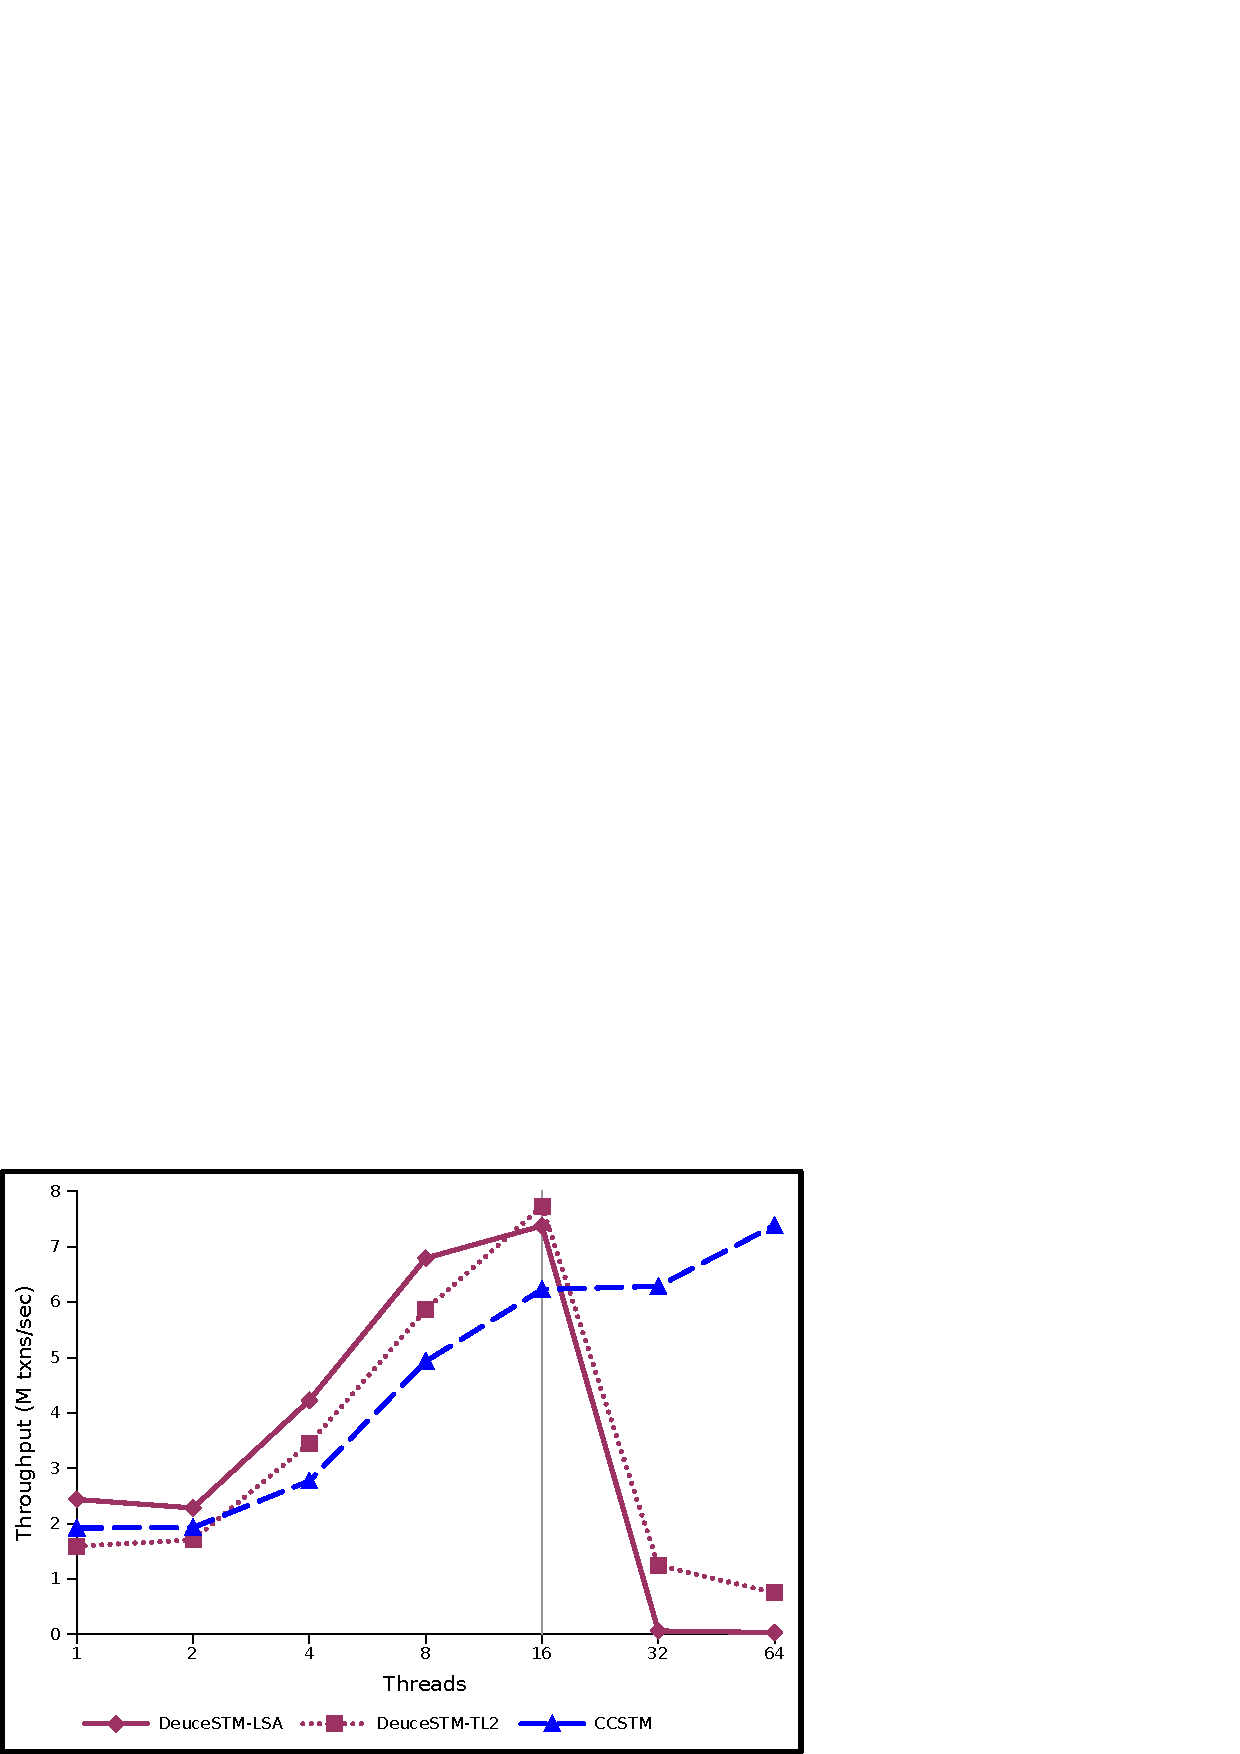
\includegraphics[clip=true,width=3in]{build/low_cont}

\caption{Throughput for the bank benchmark in a low contention scenario,
on a machine with 16 hardware thread contexts.  The number of accounts
is 64 times the number of threads.}

  \label{fig:lowcont}
\end{figure}

\begin{figure}
  \centering 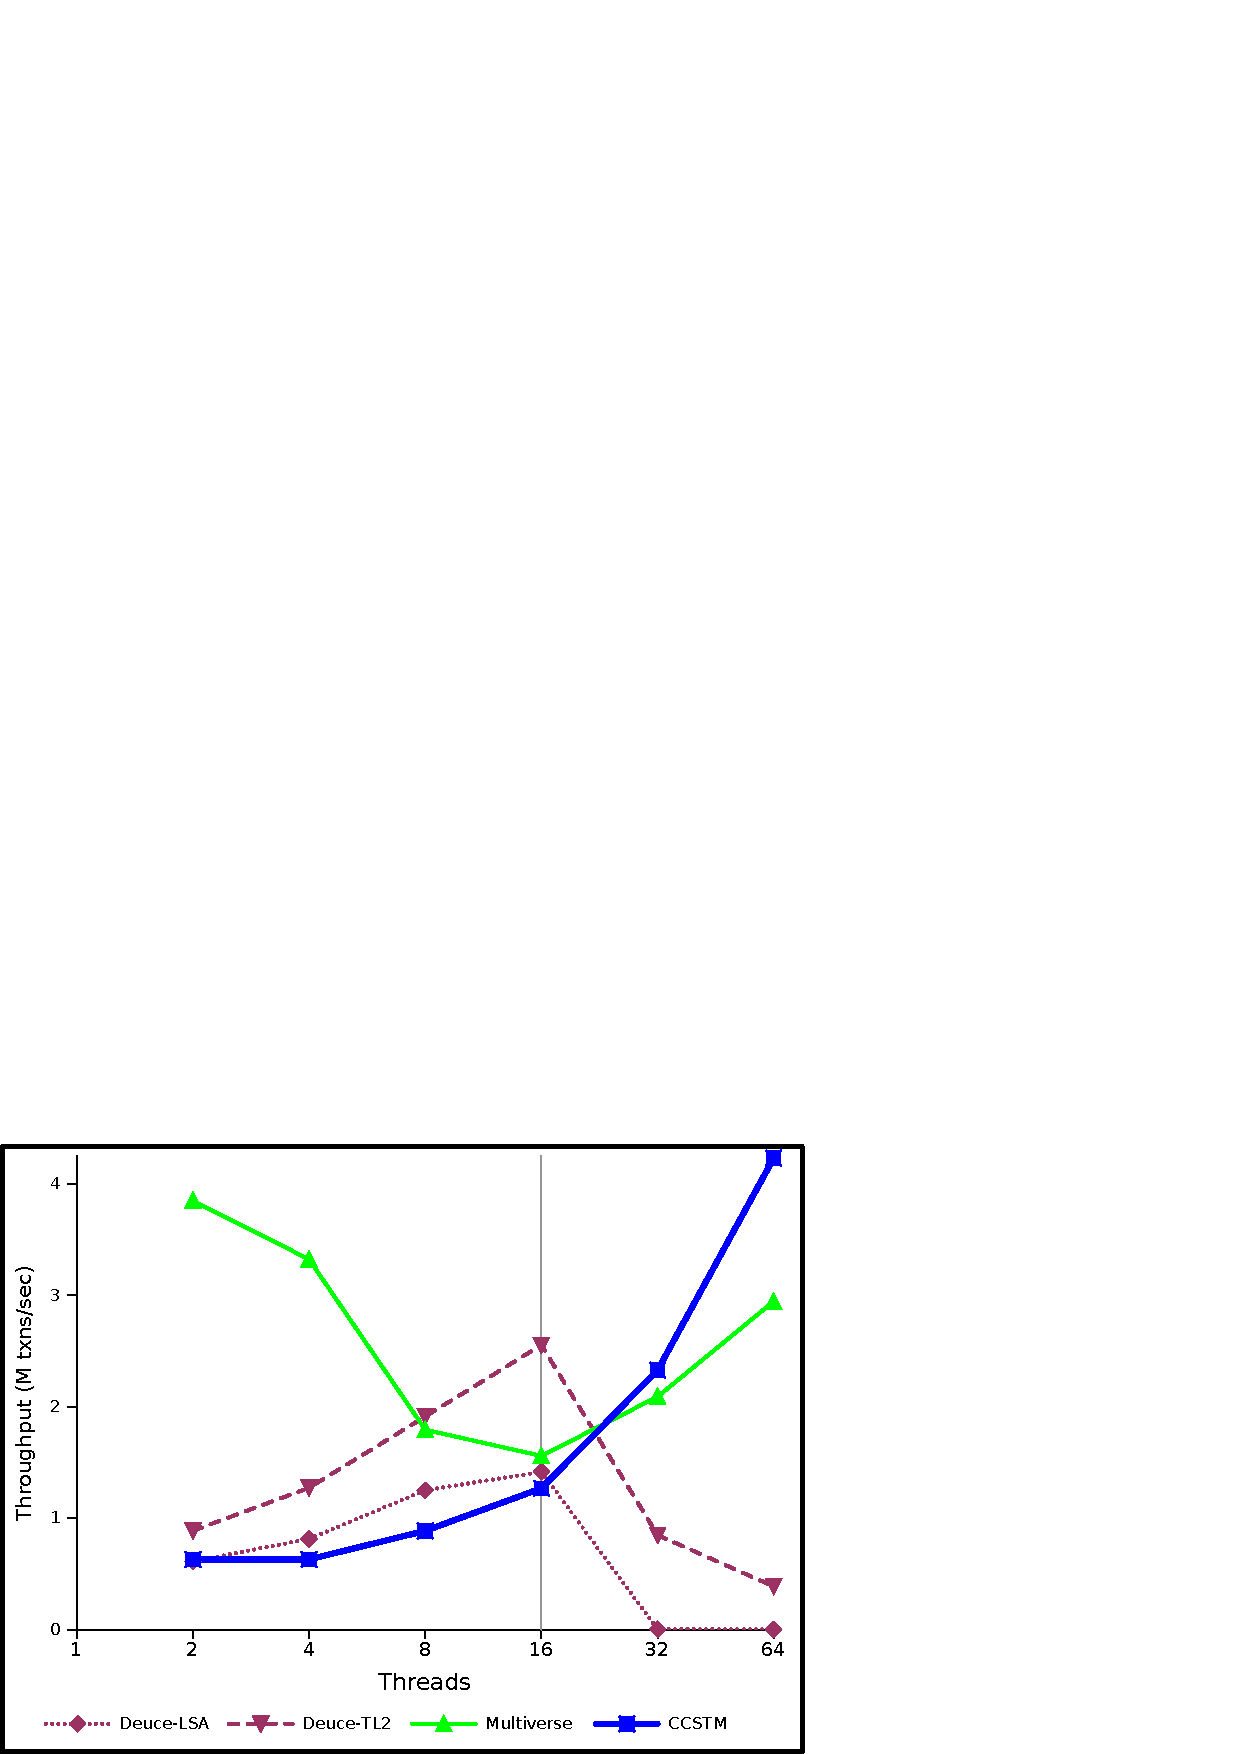
\includegraphics[clip=true,width=3in]{build/high_cont}

\caption{Throughput for a high contention scenario.  The number of accounts is
equal to the number of threads.  Each transaction touches two accounts.}

  \label{fig:highcont}
\end{figure}

CCSTM's implementation as an unprivileged library introduces several possible inefficiencies:
\type{Ref} adds a level of indirection;
JVM erasure adds boxing overheads for \xtype{Ref}{T} when \typeparam{T} is a
primitive type; dynamic scoping involves a hash table lookup, either implicitly
inside \type{ThreadLocal} or explicitly with a \type{Thread} key; low-level
atomic operations performed by the STM cannot use the unchecked primitives in
\code{sun.misc.Unsafe}; \todo{more}

must use \type{ThreadLocal} or a map keyed on
\type{Thread}, both of which add a hash table lookup , which is slower
than adding a field to the underlying thread instance.


To verify that CCSTM's library-based design does not impose a prohibitive
performance penalty, we compared it to Deuce STM and Multiverse, STMs for
the JVM that perform bytecode rewriting during class
loading~\cite{deucestm,multiverse}.

Experiments were run on a Dell Precision T7500n with two quad-core
2.66Ghz Intel Xeon X5550 processors, and 24GB of RAM.  Hyper-Threading was
enabled, yielding a total of 16 hardware thread contexts.  We used Scala
version 2.8.0.Beta1.  We ran our experiments in
Sun's Java~SE Runtime Environment, build 1.6.0\_16-b01, using the HotSpot
64-Bit Server VM.  Deuce STM was version 1.3.0.  Multiverse was version 0.4.
%We enabled dynamic escape analysis and compressed
%oops.

We performed a direct encoding of Deuce STM's bank benchmark into
Scala+CCSTM, and compared this version to the Java original running
under the bytecode rewriting STMs.  (While the example code in this paper uses an
immutable \type{Money} numeric type, the evaluated benchmark uses 32-bit
floating point values like the original.)  Deuce STM provides two algorithms,
TL2 and LSA.  In addition, it allows an optional contention manager to
be used.  For each run, we report the throughput of a Deuce STM algorithm
as the maximum of the throughput with or without contention management.
For almost all configurations we tested, contention management reduced
throughput.  CCSTM and Multiverse were tested using their default
configuration.

This benchmark includes its own harness, which we configured so
that no overdrafts were triggered.  We used a 4 second warmup, and
then measured the number of transactions committed during 10 seconds,
averaging across three invocations of the JVM.  For the low-contention
experiment (Figure~\ref{fig:lowcont}) we set the number of accounts
to 64 times the number of threads.  For the high-contention experiment
(Figure~\ref{fig:highcont}) we set the number of accounts to the number of
threads.  Single-threaded execution is not included in the high-contention
setup, as it has no contention.  Because at most 16 threads are executing
at any time, high-contention runs have fewer conflicts at 32 and 64
threads than for lower thread counts, and so can continue to scale.

\todo{talk about multiverse}
The TL2 version of Deuce STM is faster than CCSTM for both experiments when
the multi-threading level is less than or equal to one.  The difference
is largest for the high-contention scenario, where threads are often
obstructed.  Deuce STM does not block threads that cannot proceed, and it
does not even use sleeps or yields.  This strategy works well when every
thread gets its own hardware context, but results in a catastrophic
performance dropoff for higher thread counts.  CCSTM's synchronization
implementation is more expensive, but yields stable performance even at
high multi-threading levels.

Deuce STM and CCSTM have different algorithms and engineering tradeoffs,
so these experiments do not allow us to exactly measure the overhead
imposed by the library-only design.  They do demonstrate, however,
that any overhead that does exist is small enough to be tolerable.


\section{Conclusion and future direction}
\label{sec:conclusion}

STM's high level programming model addresses many of the challenges of
shared memory multithreading, but to be most useful its benefits should
be provided in a pay-as-you-go fashion.  CCSTM accomplishes this by
providing transactional memory as a normal Scala library.

CCSTM uses Scala's features to embed STM as a DSL, rather than using
bytecode rewriting or VM modifications to transparently redirect loads and
stores.  Its syntax is concise, and its performance is on par
with bytecode rewriting STMs.  The references that encapsulate
transactionally-managed memory locations add some clutter to the user's
code, but they also provide a natural way for the programmer to take
advantage of more sophisticated features such as semantic conflict
detection.  The implementation is careful to avoid busy-waiting or
polling when a transaction is blocked, delivering good performance
despite contention and high multithreading levels.  CCSTM demonstrates
that a library-based STM can be usable and performant.



\appendix
\section{Code}

Source code for CCSTM is available under a BSD license from
\textsf{http://github.com/nbronson/ccstm}.

%%This is the text of the appendix, if you need one.

\acks

The authors would like to specifically thank Daniel Spiewak and Peter
Veentjer for their helpful feedback during the design phase of CCSTM.

This work was supported by the Stanford Pervasive Parallelism Lab,
by Dept. of the Army, AHPCRC W911NF-07-2-0027-1, and by
the National Science Foundation under grant CNS--0720905.

{
%\small
\bibliographystyle{abbrv}
%\bibliographystyle{plainnat}
%\renewcommand{\bibfont}{\normalsize}
\bibliography{../../common/ppl}

%\begin{thebibliography}{10}
%\end{thebibliography}
}

\end{document}

